\newpage
\subsection{Caso d'uso UC14: Amministrazione applicazione web}
\label{UC14}
\begin{figure}[ht]
	\centering
	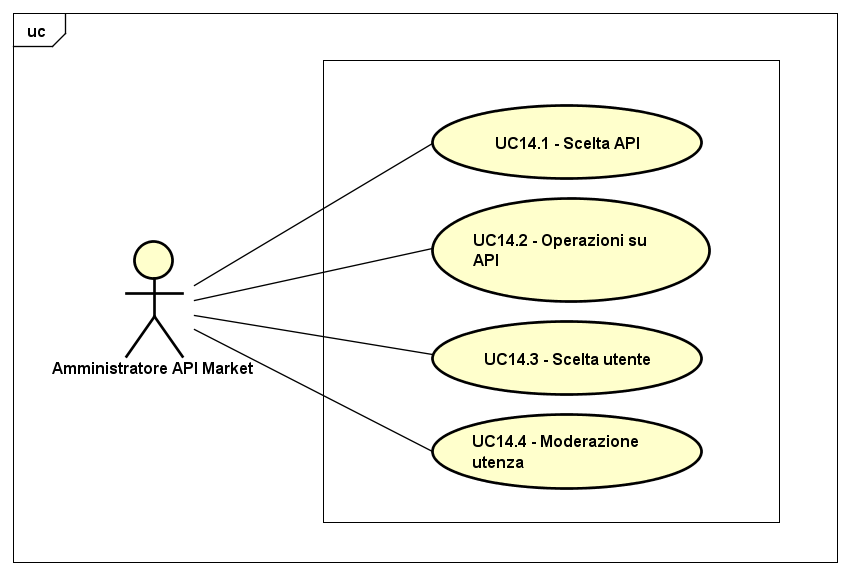
\includegraphics[scale=0.45]{UML/UC14.png}
	\caption{UC14 - Amministrazione applicazione web}
\end{figure}

\begin{longtable}{ l | p{11cm}}
	\hline
	\rowcolor{Gray}
	\multicolumn{2}{c}{UC14: Amministrazione applicazione web} \\
	\hline
	\textbf{Attori} & Amministratore API Market \\
	\textbf{Descrizione} & L'attore amministra l'applicazione web e/o consulta i dati di utilizzo avanzati \\
	\textbf{Pre-Condizioni} & L'attore si trova nella schermata iniziale dell'applicazione web \\
	\textbf{Post-Condizioni} & L'attore ha amministrato l'applicazione web e/o ha consultato i dati di utilizzo avanzati \\
	\textbf{Scenario Principale} & 
	\begin{enumerate*}[label=(\arabic*.),itemjoin={\newline}]
		\item L'attore può scegliere una API (UC14.1)
		\item L'attore può eseguire delle operazioni sull'API scelta (UC14.2)
		\item L'attore può scegliere un utente (UC14.3)
		\item L'attore può moderare l'utente scelto (UC14.4)
	\end{enumerate*}\\
\end{longtable}

\subsubsection{Caso d'uso UC14.1: Scelta API}
\label{UC14_1}

\begin{minipage}{\linewidth}
	\begin{tabular}{ l | p{11cm}}
		\hline
		\rowcolor{Gray}
		\multicolumn{2}{c}{UC14.1 - Scelta API} \\
		\hline
		\textbf{Attori} & Amministratore API Market \\
		\textbf{Descrizione} & L'attore sceglie una API su cui effettuare delle operazioni \\
		\textbf{Pre-Condizioni} & L'attore si trova nella schermata relativa all'amministrazione dell'applicazione web \\
		\textbf{Post-Condizioni} & L'attore ha scelto una API su cui effettuare delle operazioni \\
		\textbf{Scenario Principale} & 
		\begin{enumerate*}[label=(\arabic*.),itemjoin={\newline}]
			\item L'attore può scegliere una API su cui effettuare delle operazioni
		\end{enumerate*}\\
	\end{tabular}
\end{minipage}

\newpage
\subsubsection{Caso d'uso UC14.2: Operazioni su API}
\label{UC14_2}
\begin{figure}[ht]
	\centering
	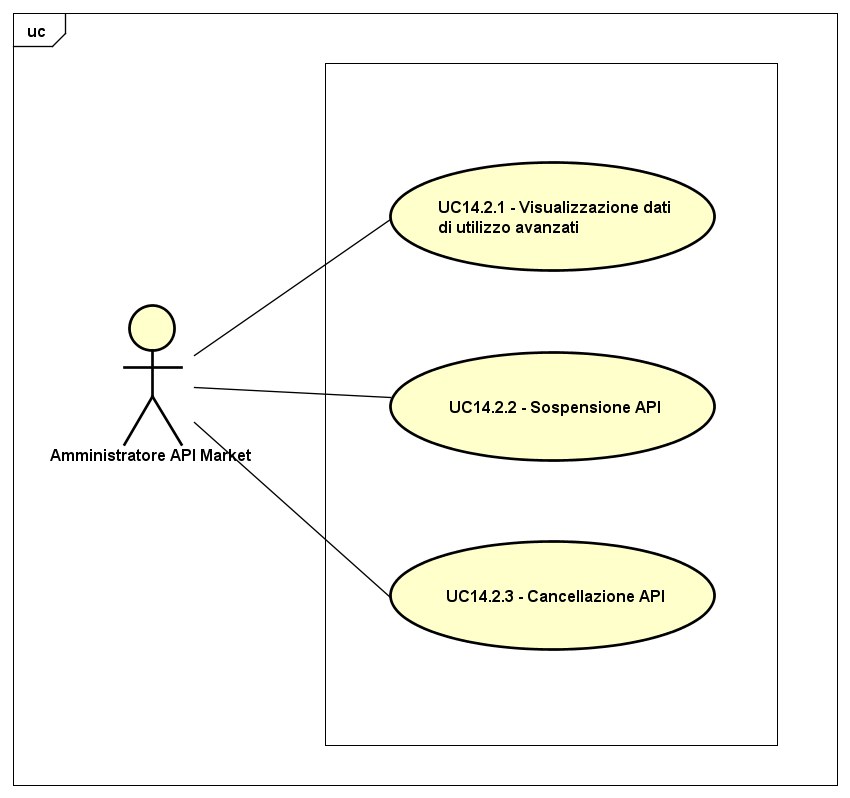
\includegraphics[scale=0.45]{UML/UC14_2.png}
	\caption{UC14.2: Operazioni su API}
\end{figure}

\begin{minipage}{\linewidth}
	\begin{tabular}{ l | p{11cm}}
		\hline
		\rowcolor{Gray}
		\multicolumn{2}{c}{UC14.2 - Operazioni su API} \\
		\hline
		\textbf{Attori} &  Amministratore API Market \\
		\textbf{Descrizione} & L'attore esegue le operazioni sull'API scelta \\
		\textbf{Pre-Condizioni} & L'attore si trova nella schermata relativa all'amministrazione dell'applicazione web ed ha scelto una API su cui operare \\
		\textbf{Post-Condizioni} & L'attore ha concluso le operazioni sull'API \\
		\textbf{Scenario Principale} & 
		\begin{enumerate*}[label=(\arabic*.),itemjoin={\newline}]
			\item L'attore può visualizzare i dati avanzati dell'API (UC14.2.1)
			\item L'attore può sospendere il funzionamento dell'API (UC14.2.2)
			\item L'attore può cancellare l'API da API Market (UC14.2.3)
		\end{enumerate*}\\
	\end{tabular}
\end{minipage}

\newpage
\paragraph{Caso d'uso UC14.2.1: Visualizzazione dati di utilizzo avanzati}
\label{UC14_2_1}
\begin{figure}[ht]
	\centering
	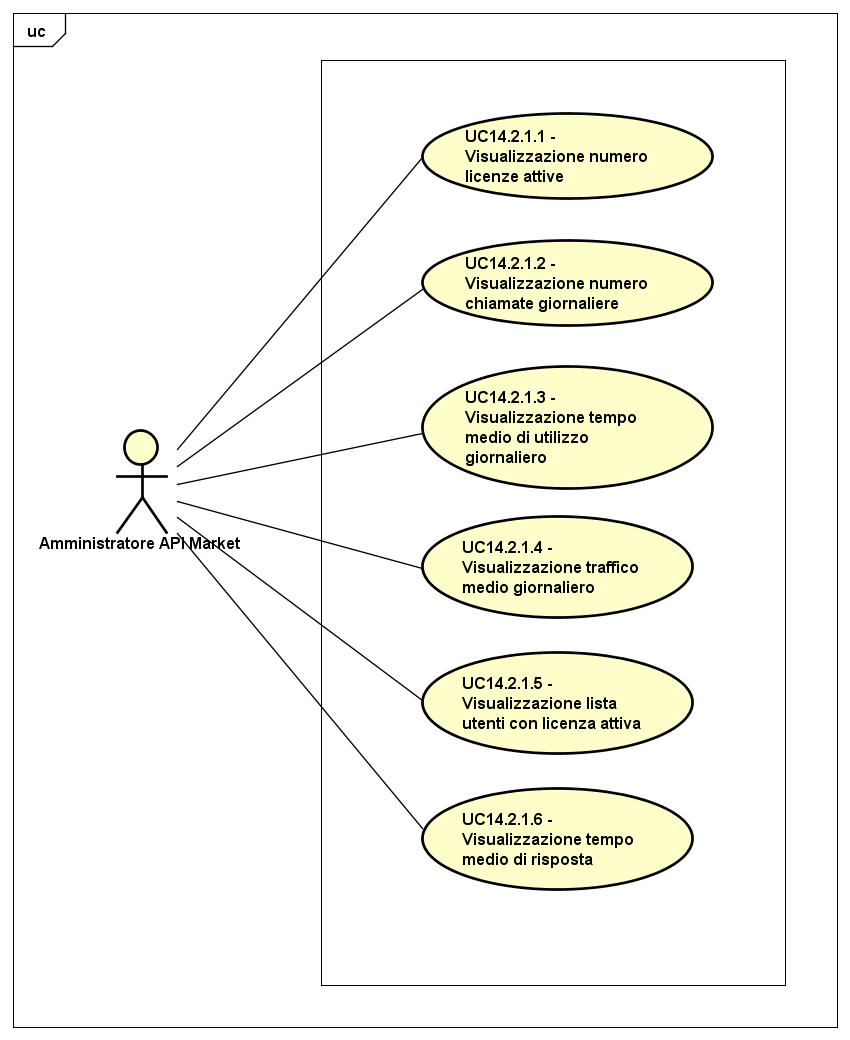
\includegraphics[scale=0.45]{UML/UC14_2_1.png}
	\caption{UC14.2.1: Visualizzazione dati di utilizzo avanzati}
\end{figure}

\begin{minipage}{\linewidth}
	\begin{tabular}{ l | p{11cm}}
		\hline
		\rowcolor{Gray}
		\multicolumn{2}{c}{UC14.2.1 - Visualizzazione dati di utilizzo avanzati} \\
		\hline
		\textbf{Attori} &  Amministratore API Market \\
		\textbf{Descrizione} & L'attore sceglie una API e ne visualizza i dati di utilizzo avanzati \\
		\textbf{Pre-Condizioni} & L'attore si trova nella schermata relativa all'amministrazione dell'applicazione web ed ha scelto una API su cui operare \\
		\textbf{Post-Condizioni} & L'attore ha scelto una API e ne ha visualizzato i dati di utilizzo avanzati \\
		\textbf{Scenario Principale} & 
		\begin{enumerate*}[label=(\arabic*.),itemjoin={\newline}]
			\item L'attore può visualizzare il numero di licenze attive dell'API scelta (UC14.2.1.1)
			\item L'attore può visualizzare il numero di chiamate giornaliere effettuate all'API scelta (UC14.2.1..2)
			\item L'attore può visualizzare il tempo medio di utilizzo giornaliero dell'API scelta (UC14.2.1.3)
			\item L'attore può visualizzare il traffico medio giornaliero dell'API scelta (UC14.2.1.4)
			\item L'attore può visualizzare la lista degli utenti con una licenza attiva per l'API scelta (UC14.2.1.5)
			\item L'attore può visualizzare il tempo medio di risposta dell'API scelta (UC14.2.1.6)
		\end{enumerate*}\\
	\end{tabular}
\end{minipage}

\subparagraph{Caso d'uso UC14.2.1.1: Visualizzazione numero licenze attive}
\label{UC14_2_1_1}

\begin{minipage}{\linewidth}
	\begin{tabular}{ l | p{11cm}}
		\hline
		\rowcolor{Gray}
		\multicolumn{2}{c}{UC14.2.1.1 - Visualizzazione numero licenze attive} \\
		\hline
		\textbf{Attori} & Amministratore API Market \\
		\textbf{Descrizione} & L'attore visualizza il numero di licenze attive per l'API scelta \\
		\textbf{Pre-Condizioni} & L'attore si trova nella schermata relativa all'amministrazione dell'applicazione web ed ha scelto una API su cui operare \\
		\textbf{Post-Condizioni} & L'attore ha visualizzato il numero di licenze attive per l'API scelta \\
		\textbf{Scenario Principale} & 
		\begin{enumerate*}[label=(\arabic*.),itemjoin={\newline}]
			\item L'attore può visualizzare il numero di licenze attive per l'API scelta
		\end{enumerate*}\\
	\end{tabular}
\end{minipage}

\subparagraph{Caso d'uso UC14.2.1.2: Visualizzazione numero chiamate giornaliere}
\label{UC14_2_1_2}

\begin{minipage}{\linewidth}
	\begin{tabular}{ l | p{11cm}}
		\hline
		\rowcolor{Gray}
		\multicolumn{2}{c}{UC14.2.1.2 - Visualizzazione numero chiamate giornaliere} \\
		\hline
		\textbf{Attori} & Amministratore API Market \\
		\textbf{Descrizione} & L'attore visualizza il numero di chiamate giornaliere effettuate all'API scelta \\
		\textbf{Pre-Condizioni} & L'attore si trova nella schermata relativa all'amministrazione dell'applicazione web ed ha scelto una API su cui operare \\
		\textbf{Post-Condizioni} & L'attore ha visualizzato il numero di chiamate giornaliere effettuate all'API scelta \\
		\textbf{Scenario Principale} & 
		\begin{enumerate*}[label=(\arabic*.),itemjoin={\newline}]
			\item L'attore può visualizzare il numero di chiamate giornaliere effettuate all'API scelta
		\end{enumerate*}\\
	\end{tabular}
\end{minipage}

\subparagraph{Caso d'uso UC14.2.1.3: Visualizzazione tempo medio di utilizzo giornaliero}
\label{UC14_2_1_3}

\begin{minipage}{\linewidth}
	\begin{tabular}{ l | p{11cm}}
		\hline
		\rowcolor{Gray}
		\multicolumn{2}{c}{14.2.1.3 - Visualizzazione tempo medio di utilizzo giornaliero} \\
		\hline
		\textbf{Attori} & Amministratore API Market \\
		\textbf{Descrizione} & L'attore visualizza il tempo medio di utilizzo giornaliero dell'API scelta \\
		\textbf{Pre-Condizioni} & L'attore si trova nella schermata relativa all'amministrazione dell'applicazione web ed ha scelto una API su cui operare \\
		\textbf{Post-Condizioni} & L'attore ha visualizzato il tempo medio di utilizzo giornaliero dell'API scelta \\
		\textbf{Scenario Principale} & 
		\begin{enumerate*}[label=(\arabic*.),itemjoin={\newline}]
			\item L'attore può visualizzare il tempo medio di utilizzo giornaliero dell'API scelta
		\end{enumerate*}\\
	\end{tabular}
\end{minipage}

\subparagraph{Caso d'uso UC14.2.1.4: Visualizzazione traffico medio giornaliero}
\label{UC14_2_1_4}

\begin{minipage}{\linewidth}
	\begin{tabular}{ l | p{11cm}}
		\hline
		\rowcolor{Gray}
		\multicolumn{2}{c}{UC14.2.1.4 - Visualizzazione traffico medio giornaliero} \\
		\hline
		\textbf{Attori} & Amministratore API Market \\
		\textbf{Descrizione} & L'attore visualizza il traffico medio giornaliero dell'API scelta \\
		\textbf{Pre-Condizioni} & L'attore si trova nella schermata relativa all'amministrazione dell'applicazione web ed ha scelto una API su cui operare \\
		\textbf{Post-Condizioni} & L'attore ha visualizzato il traffico medio giornaliero dell'API scelta \\
		\textbf{Scenario Principale} & 
		\begin{enumerate*}[label=(\arabic*.),itemjoin={\newline}]
			\item L'attore può visualizzare il traffico medio giornaliero dell'API scelta
		\end{enumerate*}\\
	\end{tabular}
\end{minipage}

\newpage
\subparagraph{Caso d'uso UC14.2.1.5: Visualizzazione utenti con licenza attiva}
\label{UC14_2_1_5}
\begin{figure}[ht]
	\centering
	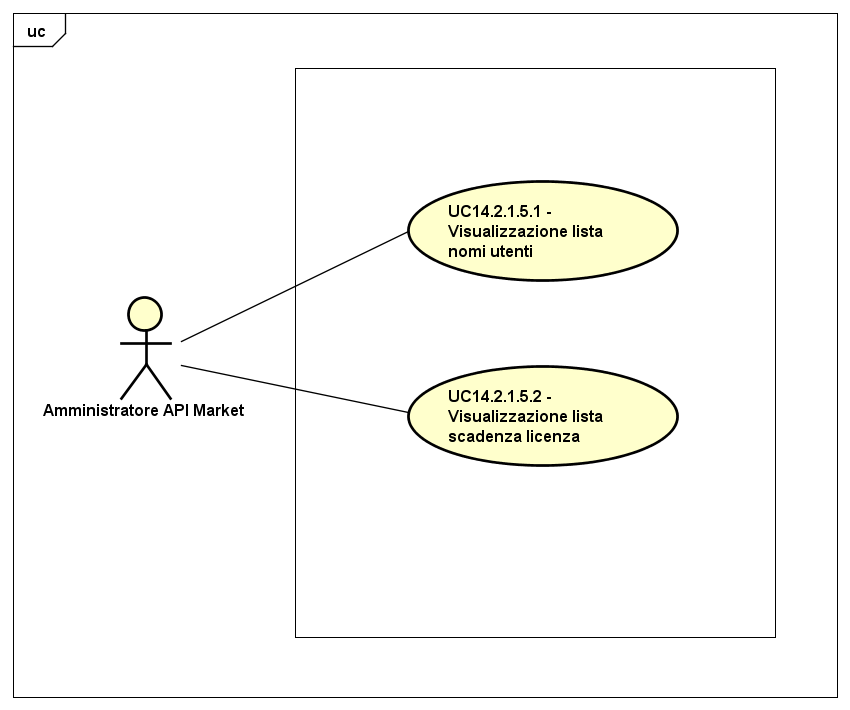
\includegraphics[scale=0.45]{UML/UC14_2_1_5.png}
	\caption{UC14.2.1.5: Visualizzazione utenti con licenza attiva}
\end{figure}

\begin{minipage}{\linewidth}
	\begin{tabular}{ l | p{11cm}}
		\hline
		\rowcolor{Gray}
		\multicolumn{2}{c}{UC14.2.1.5 - Visualizzazione utenti con licenza attiva} \\
		\hline
		\textbf{Attori} & Amministratore API Market \\
		\textbf{Descrizione} & L'attore ha scelto una API e visualizza una lista di utenti con licenze attive per l'API scelta\\
		\textbf{Pre-Condizioni} & L'attore si trova nella schermata relativa all'amministrazione dell'applicazione web ed ha scelto una API su cui operare \\
		\textbf{Post-Condizioni} & L'attore ha visualizzato la lista di utenti con licenze attive per l'API scelta \\
		\textbf{Scenario Principale} & 
		\begin{enumerate*}[label=(\arabic*.),itemjoin={\newline}]
			\item L'attore può visualizzare il nome di ogni utente con licenza attiva per l'API scelta (UC14.2.1.5.1)
			\item L'attore può visualizzare la data di scadenza della licenza per ogni utente nella lista (UC14.2.1.5.2)
		\end{enumerate*}\\
	\end{tabular}
\end{minipage}

\subparagraph{Caso d'uso UC14.2.1.5.1: Visualizzazione lista nomi utenti}
\label{UC14_2_1_5_1}

\begin{minipage}{\linewidth}
	\begin{tabular}{ l | p{11cm}}
		\hline
		\rowcolor{Gray}
		\multicolumn{2}{c}{UC14.2.1.5.1 - Visualizzazione lista nomi utenti} \\
		\hline
		\textbf{Attori} & Amministratore API Market \\
		\textbf{Descrizione} & L'attore ha scelto una API e visualizza il nome dell'utente interessato\\
		\textbf{Pre-Condizioni} & L'attore si trova nella schermata relativa all'amministrazione dell'applicazione web ed ha scelto una API su cui operare \\
		\textbf{Post-Condizioni} & L'attore ha visualizzato il nome per ogni utente della lista degli utenti con licenza attiva per l'API scelta \\
		\textbf{Scenario Principale} & 
		\begin{enumerate*}[label=(\arabic*.),itemjoin={\newline}]
			\item L'attore può visualizzare il nome per ogni utente della lista degli utenti con licenza attiva per l'API scelta
		\end{enumerate*}
	\end{tabular}
\end{minipage}

\subparagraph{Caso d'uso UC14.2.1.5.2: Visualizzazione lista scadenza licenza}
\label{UC14_2_1_5_2}

\begin{minipage}{\linewidth}
	\begin{tabular}{ l | p{11cm}}
		\hline
		\rowcolor{Gray}
		\multicolumn{2}{c}{UC14.2.1.5.2 -  Visualizzazione lista scadenza licenza} \\
		\hline
		\textbf{Attori} & Amministratore API Market \\
		\textbf{Descrizione} & L'attore ha scelto una API e visualizza il parametro di scadenza per ogni utente della lista degli utenti con licenza attiva per l'API scelta \\
		\textbf{Pre-Condizioni} & L'attore si trova nella schermata relativa all'amministrazione dell'applicazione web ed ha scelto una API su cui operare \\
		\textbf{Post-Condizioni} & L'attore ha visualizzato il parametro di scadenza per ogni utente della lista degli utenti con licenza attiva per l'API scelta \\
		\textbf{Scenario Principale} & 
		\begin{enumerate*}[label=(\arabic*.),itemjoin={\newline}]
			\item L'attore può visualizzare il parametro di scadenza per ogni utente della lista degli utenti con licenza attiva per l'API scelta
		\end{enumerate*}
	\end{tabular}
\end{minipage}

\subparagraph{Caso d'uso UC14.2.1.6: Visualizzazione tempo medio di risposta}
\label{UC14_2_1_6}

\begin{minipage}{\linewidth}
	\begin{tabular}{ l | p{11cm}}
		\hline
		\rowcolor{Gray}
		\multicolumn{2}{c}{UC14.2.1.6 - Visualizzazione tempo medio di risposta} \\
		\hline
		\textbf{Attori} & Amministratore API Market \\
		\textbf{Descrizione} & L'attore ha scelto una API e visualizza il tempo medio di risposta dell'API scelta \\
		\textbf{Pre-Condizioni} & L'attore si trova nella schermata relativa all'amministrazione dell'applicazione web ed ha scelto una API su cui operare \\
		\textbf{Post-Condizioni} & L'attore ha visualizzato il tempo medio di risposta dell'API scelta \\
		\textbf{Scenario Principale} & 
		\begin{enumerate*}[label=(\arabic*.),itemjoin={\newline}]
			\item L'attore può visualizzare il tempo medio di risposta dell'API scelta
		\end{enumerate*}\\
	\end{tabular}
\end{minipage}

\newpage
\paragraph{Caso d'uso UC14.2.2: Sospensione API}
\label{UC14_2_2}
\begin{figure}[ht]
	\centering
	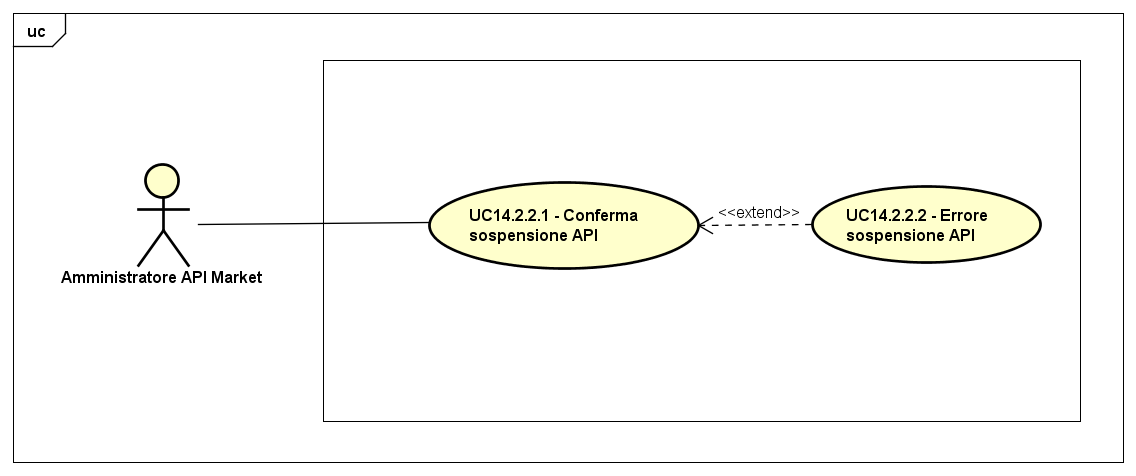
\includegraphics[scale=0.45]{UML/UC14_2_2.png}
	\caption{UC14.2.2: Sospensione API}
\end{figure}

\begin{minipage}{\linewidth}
	\begin{tabular}{ l | p{11cm}}
		\hline
		\rowcolor{Gray}
		\multicolumn{2}{c}{UC14.2.2 - Sospensione API} \\
		\hline
		\textbf{Attori} & Amministratore API Market \\
		\textbf{Descrizione} & L'attore sospende l'API scelta \\
		\textbf{Pre-Condizioni} & L'attore si trova nella schermata relativa all'amministrazione dell'applicazione web ed ha scelto una API su cui operare \\
		\textbf{Post-Condizioni} & L'attore ha sospeso l'API scelta \\
		\textbf{Scenario Principale} & 
		\begin{enumerate*}[label=(\arabic*.),itemjoin={\newline}]
			\item L'attore può confermare la sospensione dell'API scelta (UC14.2.2.1)
		\end{enumerate*}\\
		\textbf{Scenari Alternativi} & 
		\begin{enumerate*}[label=(\arabic*.),itemjoin={\newline}]
			\item L'attore, dopo aver confermato la sospensione dell'API scelta, può visualizzare un messaggio di errore informativo e la sospensione non avviene (UC14.2.2.2)
		\end{enumerate*}\\
	\end{tabular}
\end{minipage}

\subparagraph{Caso d'uso UC14.2.2.1: Conferma sospensione API}
\label{UC14_2_2_1}

\begin{minipage}{\linewidth}
	\begin{tabular}{ l | p{11cm}}
		\hline
		\rowcolor{Gray}
		\multicolumn{2}{c}{UC14.2.2.1 - Conferma sospensione API} \\
		\hline
		\textbf{Attori} & Amministratore API Market \\
		\textbf{Descrizione} & L'attore conferma la sospensione dell'utente scelto e visualizza un messaggio di successo \\
		\textbf{Pre-Condizioni} & L'attore si trova nella schermata relativa all'amministrazione dell'applicazione web ed ha scelto una API su cui operare \\
		\textbf{Post-Condizioni} & L'attore ha confermato la sospensione dell'API scelta \\
		\textbf{Scenario Principale} & 
		\begin{enumerate*}[label=(\arabic*.),itemjoin={\newline}]
			\item L'attore conferma la sospensione dell'API scelta e visualizza un messaggio di successo
		\end{enumerate*}\\
	\end{tabular}
\end{minipage}

\subparagraph{Caso d'uso UC14.2.2.2: Errore sospensione API}
\label{UC14_2_2_2}

\begin{minipage}{\linewidth}
	\begin{tabular}{ l | p{11cm}}
		\hline
		\rowcolor{Gray}
		\multicolumn{2}{c}{UC14.2.2.2 - Errore sospensione API} \\
		\hline
		\textbf{Attori} & Amministratore API Market \\
		\textbf{Descrizione} & L'attore visualizza un messaggio di errore informativo e la sospensione dell'API scelta non avviene \\
		\textbf{Pre-Condizioni} & L'attore ha confermato la sospensione dell'API scelta ma si è verificato un errore \\
		\textbf{Post-Condizioni} & L'attore ha visualizzato un messaggio di errore informativo \\
		\textbf{Scenario Principale} & 
		\begin{enumerate*}[label=(\arabic*.),itemjoin={\newline}]
			\item L'attore può visualizzare un messaggio di errore informativo e la sospensione dell'API scelta non avviene
		\end{enumerate*}\\
	\end{tabular}
\end{minipage}

\newpage
\paragraph{Caso d'uso UC14.2.3: Cancellazione API}
\label{UC14_2_3}
\begin{figure}[ht]
	\centering
	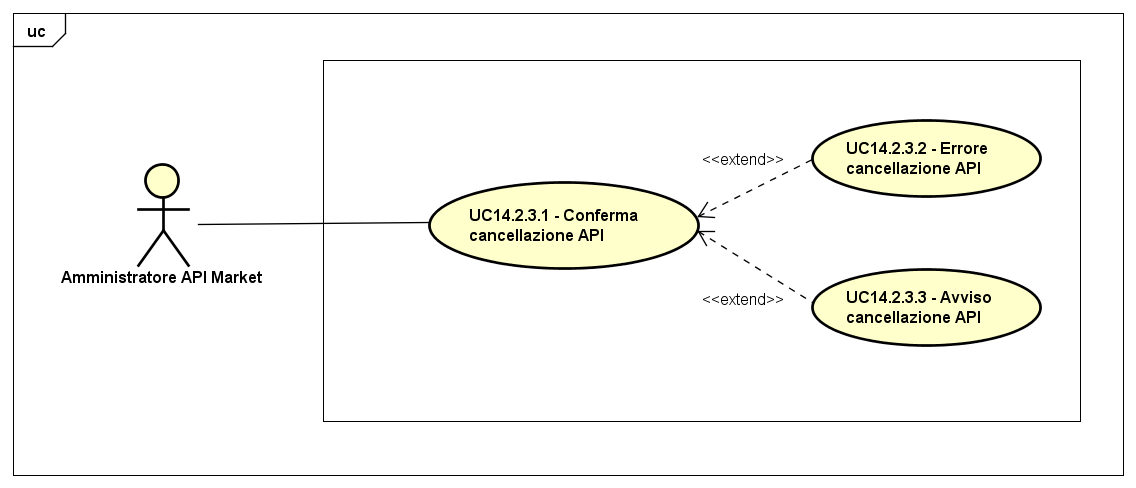
\includegraphics[scale=0.45]{UML/UC14_2_3.png}
	\caption{UC14.2.3: Cancellazione API}
\end{figure}

\begin{minipage}{\linewidth}
	\begin{tabular}{ l | p{11cm}}
		\hline
		\rowcolor{Gray}
		\multicolumn{2}{c}{UC14.2.3 - Cancellazione API} \\
		\hline
		\textbf{Attori} & Amministratore API Market \\
		\textbf{Descrizione} & L'attore cancella l'API scelta \\
		\textbf{Pre-Condizioni} & L'attore si trova nella schermata relativa all'amministrazione dell'applicazione web ed ha scelto una API su cui operare \\
		\textbf{Post-Condizioni} & L'attore ha cancellato l'API scelta \\
		\textbf{Scenario Principale} & 
		\begin{enumerate*}[label=(\arabic*.),itemjoin={\newline}]
			\item L'attore può confermare la cancellazione dell'API scelta (UC14.2.3.1)
		\end{enumerate*}\\
		\textbf{Scenari Alternativi} & 
		\begin{enumerate*}[label=(\arabic*.),itemjoin={\newline}]
			\item L'attore, dopo aver confermato la cancellazione dell'API scelta, può visualizzare un messaggio di errore informativo e la cancellazione non avviene (UC14.2.3.2)
			\item L'attore, dopo aver confermato la cancellazione dell'API scelta, può visualizzare un messaggio di avviso (E.g: Almeno una chiave API è ancora valida) e può riconfermare la cancellazione oppure abbandonarla (UC14.2.3.3)
		\end{enumerate*}\\
	\end{tabular}
\end{minipage}

\subparagraph{Caso d'uso UC14.2.3.1: Conferma cancellazione API}
\label{UC14_2_3_1}

\begin{minipage}{\linewidth}
	\begin{tabular}{ l | p{11cm}}
		\hline
		\rowcolor{Gray}
		\multicolumn{2}{c}{UC14.2.3.1 - Conferma cancellazione API} \\
		\hline
		\textbf{Attori} & Amministratore API Market \\
		\textbf{Descrizione} & L'attore conferma la cancellazione dell'utente scelto e visualizza un messaggio di successo \\
		\textbf{Pre-Condizioni} & L'attore si trova nella schermata relativa all'amministrazione dell'applicazione web ed ha scelto una API su cui operare \\
		\textbf{Post-Condizioni} & L'attore ha confermato la cancellazione dell'API scelta \\
		\textbf{Scenario Principale} & 
		\begin{enumerate*}[label=(\arabic*.),itemjoin={\newline}]
			\item L'attore conferma la cancellazione dell'API scelta e visualizza un messaggio di successo
		\end{enumerate*}\\
	\end{tabular}
\end{minipage}

\subparagraph{Caso d'uso UC14.2.3.2: Errore cancellazione API}
\label{UC14_2_3_2}

\begin{minipage}{\linewidth}
	\begin{tabular}{ l | p{11cm}}
		\hline
		\rowcolor{Gray}
		\multicolumn{2}{c}{UC14.2.3.2 - Errore cancellazione API} \\
		\hline
		\textbf{Attori} & Amministratore API Market \\
		\textbf{Descrizione} & L'attore visualizza un messaggio di errore informativo e la cancellazione dell'API scelta non avviene \\
		\textbf{Pre-Condizioni} & L'attore ha confermato la cancellazione dell'API scelta ma si è verificato un errore \\
		\textbf{Post-Condizioni} & L'attore ha visualizzato un messaggio di errore informativo \\
		\textbf{Scenario Principale} & 
		\begin{enumerate*}[label=(\arabic*.),itemjoin={\newline}]
			\item L'attore può visualizzare un messaggio di errore informativo e la cancellazione dell'API scelta non avviene
		\end{enumerate*}\\
	\end{tabular}
\end{minipage}

\subparagraph{Caso d'uso UC14.2.3.3: Avviso cancellazione API}
\label{UC14_2_3_3}

\begin{minipage}{\linewidth}
	\begin{tabular}{ l | p{11cm}}
		\hline
		\rowcolor{Gray}
		\multicolumn{2}{c}{UC14.2.3.3 - Avviso cancellazione API} \\
		\hline
		\textbf{Attori} & Amministratore API Market \\
		\textbf{Descrizione} & L'attore visualizza un messaggio di avviso e sceglie se riconfermare la cancellazione dell'API \\
		\textbf{Pre-Condizioni} & L'attore ha confermato la cancellazione dell'API scelta ma si è verificato un errore \\
		\textbf{Post-Condizioni} & L'attore ha visualizzato un messaggio di avviso ed ha scelto se riconfermare la cancellazione dell'API \\
		\textbf{Scenario Principale} & 
		\begin{enumerate*}[label=(\arabic*.),itemjoin={\newline}]
			\item L'attore può visualizzare un messaggio di avviso e scegliere se riconfermare la cancellazione dell'API
		\end{enumerate*}\\
	\end{tabular}
\end{minipage}

\subsubsection{Caso d'uso UC14.3: Scelta utente}
\label{UC14_3}

\begin{minipage}{\linewidth}
	\begin{tabular}{ l | p{11cm}}
		\hline
		\rowcolor{Gray}
		\multicolumn{2}{c}{UC14.3 - Scelta utente} \\
		\hline
		\textbf{Attori} & Amministratore API Market \\
		\textbf{Descrizione} & L'attore sceglie un utente da moderare \\
		\textbf{Pre-Condizioni} & L'attore si trova nella schermata relativa all'amministrazione dell'applicazione web \\
		\textbf{Post-Condizioni} & L'attore ha scelto un utente da moderare \\
		\textbf{Scenario Principale} & 
		\begin{enumerate*}[label=(\arabic*.),itemjoin={\newline}]
			\item L'attore può scegliere un utente da moderare
		\end{enumerate*}\\
	\end{tabular}
\end{minipage}

\newpage
\subsubsection{Caso d'uso UC14.4: Moderazione utenza}
\label{UC14_4}
\begin{figure}[ht]
	\centering
	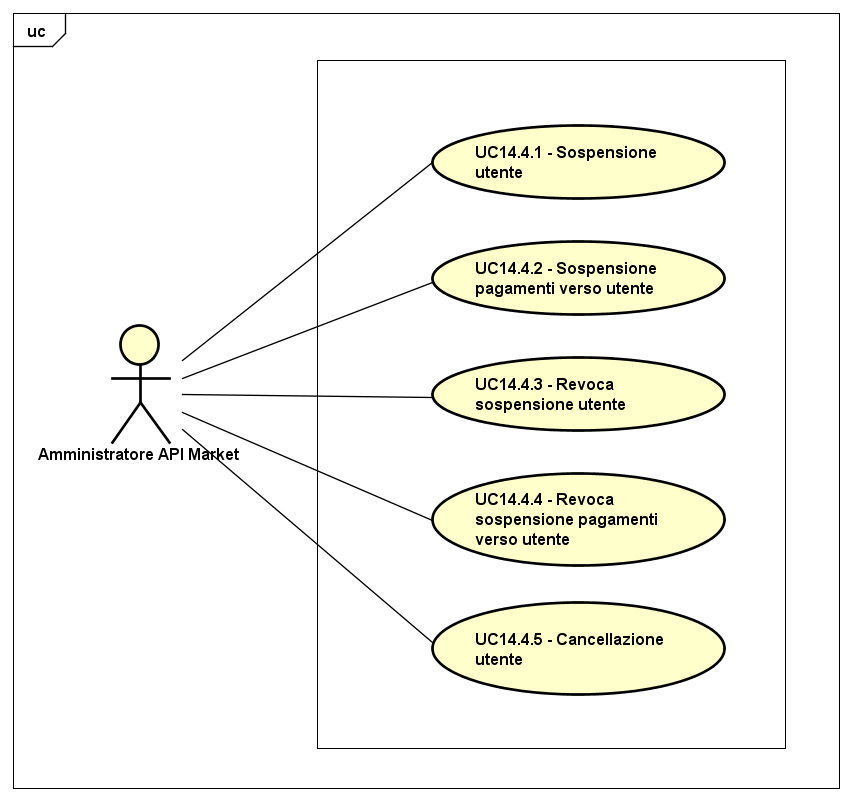
\includegraphics[scale=0.45]{UML/UC14_4.png}
	\caption{UC14.4: Moderazione utenza}
\end{figure}

\begin{minipage}{\linewidth}
	\begin{tabular}{ l | p{11cm}}
		\hline
		\rowcolor{Gray}
		\multicolumn{2}{c}{UC14.4 - Moderazione utenza} \\
		\hline
		\textbf{Attori} &  Amministratore API Market \\
		\textbf{Descrizione} & L'attore attua l'opera di moderazione sull'utente scelto \\
		\textbf{Pre-Condizioni} & L'attore si trova nella schermata relativa all'amministrazione dell'applicazione web ed ha scelto un utente da moderare \\
		\textbf{Post-Condizioni} & L'attore ha concluso l'opera di moderazione \\
		\textbf{Scenario Principale} & 
		\begin{enumerate*}[label=(\arabic*.),itemjoin={\newline}]
			\item L'attore può sospendere l'utente scelto (UC14.4.1)
			\item L'attore può sospendere i pagamenti verso l'utente scelto (UC14.4.2)
			\item L'attore può revocare la sospensione dell'utente scelto (UC14.4.3)
			\item L'attore può revocare la sospensione dei pagamenti verso l'utente scelto (UC14.4.4)
		\end{enumerate*}\\
	\end{tabular}
\end{minipage}

\newpage
\paragraph{Caso d'uso UC14.4.1: Sospensione utente}
\label{UC14_4_1}
\begin{figure}[ht]
	\centering
	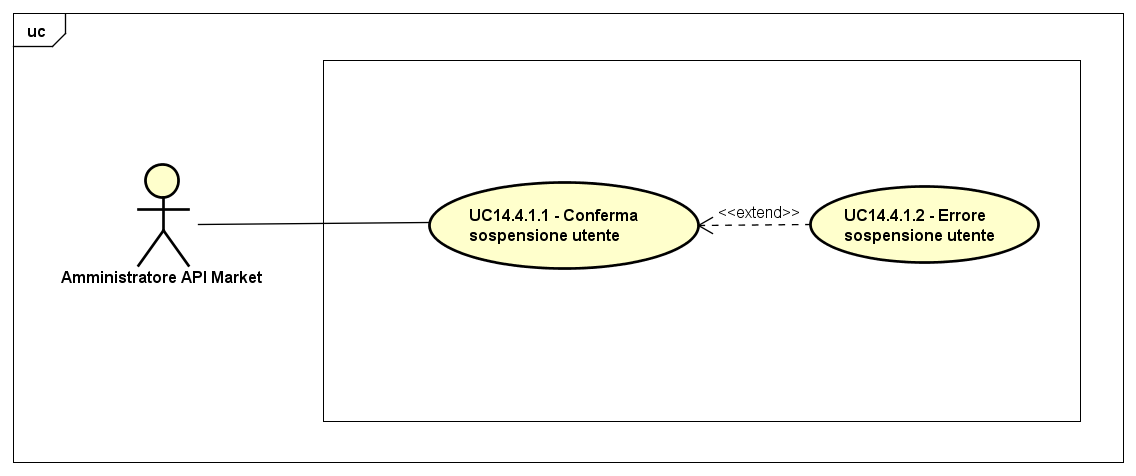
\includegraphics[scale=0.45]{UML/UC14_4_1.png}
	\caption{UC14.4.1: Sospensione utente}
\end{figure}

\begin{minipage}{\linewidth}
	\begin{tabular}{ l | p{11cm}}
		\hline
		\rowcolor{Gray}
		\multicolumn{2}{c}{UC14.4.1 - Sospensione utente} \\
		\hline
		\textbf{Attori} & Amministratore API Market \\
		\textbf{Descrizione} & L'attore sospende l'utente scelto (impedisce da parte sua l'uso delle API acquistate, e da parte degli altri utente l'uso delle API da lui registrate) \\
		\textbf{Pre-Condizioni} & L'attore si trova nella schermata relativa all'amministrazione dell'applicazione web ed ha scelto un utente da moderare \\
		\textbf{Post-Condizioni} & L'attore ha sospeso l'utente scelto \\
		\textbf{Scenario Principale} & 
		\begin{enumerate*}[label=(\arabic*.),itemjoin={\newline}]
			\item L'attore può confermare la sospensione dell'utente scelto (UC14.4.1.1)
		\end{enumerate*}\\
		\textbf{Scenari Alternativi} & 
		\begin{enumerate*}[label=(\arabic*.),itemjoin={\newline}]
			\item L'attore, dopo aver confermato la sospensione dell'utente scelto, può visualizzare un messaggio di errore informativo e la sospensione non avviene (UC14.4.1.2)
		\end{enumerate*}\\
	\end{tabular}
\end{minipage}

\subparagraph{Caso d'uso UC14.4.1.1: Conferma sospensione utente}
\label{UC14_4_1_1}

\begin{minipage}{\linewidth}
	\begin{tabular}{ l | p{11cm}}
		\hline
		\rowcolor{Gray}
		\multicolumn{2}{c}{UC14.4.1.1 - Conferma sospensione utente} \\
		\hline
		\textbf{Attori} & Amministratore API Market \\
		\textbf{Descrizione} & L'attore conferma la sospensione dell'utente scelto e visualizza un messaggio di successo \\
		\textbf{Pre-Condizioni} & L'attore si trova nella schermata relativa all'amministrazione dell'applicazione web ed ha scelto un utente da moderare \\
		\textbf{Post-Condizioni} & L'attore ha confermato la sospensione dell'utente scelto \\
		\textbf{Scenario Principale} & 
		\begin{enumerate*}[label=(\arabic*.),itemjoin={\newline}]
			\item L'attore conferma la sospensione dell'utente scelto e visualizza un messaggio di successo
		\end{enumerate*}\\
	\end{tabular}
\end{minipage}

\subparagraph{Caso d'uso UC14.4.1.2: Errore sospensione utente}
\label{UC14_4_1_2}

\begin{minipage}{\linewidth}
	\begin{tabular}{ l | p{11cm}}
		\hline
		\rowcolor{Gray}
		\multicolumn{2}{c}{UC14.4.1.2 - Errore sospensione utente} \\
		\hline
		\textbf{Attori} & Amministratore API Market \\
		\textbf{Descrizione} & L'attore visualizza un messaggio di errore informativo e la sospensione dell'utente scelto non avviene \\
		\textbf{Pre-Condizioni} & L'attore ha confermato la sospensione dell'utente scelto ma si è verificato un errore \\
		\textbf{Post-Condizioni} & L'attore ha visualizzato un messaggio di errore informativo \\
		\textbf{Scenario Principale} & 
		\begin{enumerate*}[label=(\arabic*.),itemjoin={\newline}]
			\item L'attore può visualizzare un messaggio di errore informativo e la sospensione dell'utente scelto non avviene
		\end{enumerate*}\\
	\end{tabular}
\end{minipage}

\newpage
\paragraph{Caso d'uso UC14.4.2: Sospensione pagamenti verso utente}
\label{UC14_4_2}
\begin{figure}[ht]
	\centering
	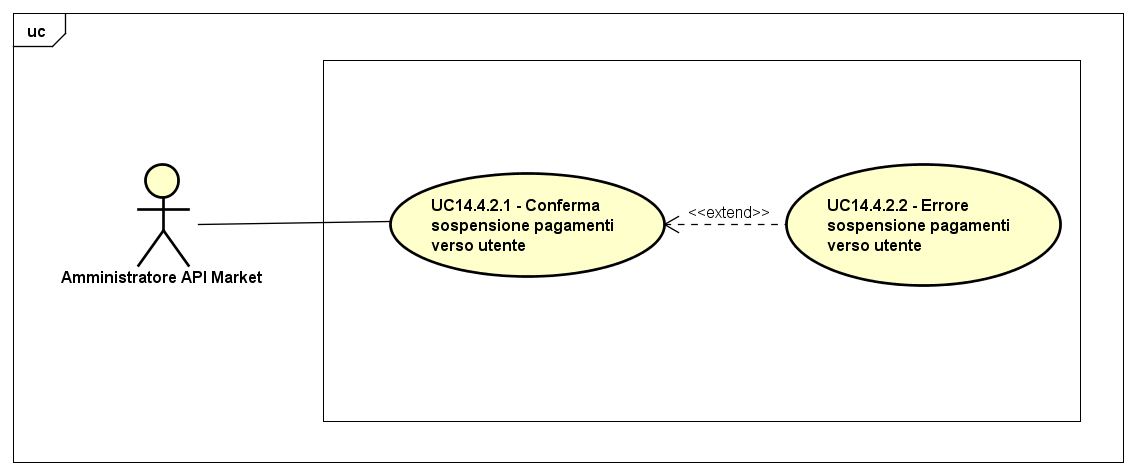
\includegraphics[scale=0.45]{UML/UC14_4_2.png}
	\caption{UC14.4.2: Sospensione pagamenti verso utente}
\end{figure}

\begin{minipage}{\linewidth}
	\begin{tabular}{ l | p{11cm}}
		\hline
		\rowcolor{Gray}
		\multicolumn{2}{c}{UC14.4.2 - Sospensione pagamenti verso utente} \\
		\hline
		\textbf{Attori} & Amministratore API Market \\
		\textbf{Descrizione} & L'attore sospende i pagamenti verso l'utente scelto \\
		\textbf{Pre-Condizioni} & L'attore si trova nella schermata relativa all'amministrazione dell'applicazione web ed ha scelto un utente da moderare \\
		\textbf{Post-Condizioni} & L'attore ha sospeso i pagamenti verso l'utente scelto \\
		\textbf{Scenario Principale} & 
		\begin{enumerate*}[label=(\arabic*.),itemjoin={\newline}]
			\item L'attore può sospendere i pagamenti verso l'utente scelto (UC14.4.2.1)
		\end{enumerate*}\\
		\textbf{Scenari Alternativi} & 
		\begin{enumerate*}[label=(\arabic*.),itemjoin={\newline}]
			\item L'attore, dopo aver confermato la sospensione dei pagamenti verso l'utente scelto, può visualizzare un messaggio di errore informativo e la sospensione dei pagamenti non avviene (UC14.4.2.2)
		\end{enumerate*}\\
	\end{tabular}
\end{minipage}

\subparagraph{Caso d'uso UC14.4.2.1: Conferma sospensione pagamenti verso utente}
\label{UC14_4_2_1}

\begin{minipage}{\linewidth}
	\begin{tabular}{ l | p{11cm}}
		\hline
		\rowcolor{Gray}
		\multicolumn{2}{c}{UC14.4.2.1 - Conferma sospensione pagamenti verso utente} \\
		\hline
		\textbf{Attori} & Amministratore API Market \\
		\textbf{Descrizione} & L'attore conferma la sospensione dei pagamenti verso l'utente scelto e visualizza un messaggio di successo \\
		\textbf{Pre-Condizioni} & L'attore si trova nella schermata relativa all'amministrazione dell'applicazione web ed ha scelto un utente da moderare \\
		\textbf{Post-Condizioni} & L'attore ha confermato la sospensione dei pagamenti verso l'utente scelto \\
		\textbf{Scenario Principale} & 
		\begin{enumerate*}[label=(\arabic*.),itemjoin={\newline}]
			\item L'attore conferma la sospensione dei pagamenti verso l'utente scelto e visualizza un messaggio di successo
		\end{enumerate*}\\
	\end{tabular}
\end{minipage}

\subparagraph{Caso d'uso UC14.4.2.2: Errore sospensione pagamenti verso utente}
\label{UC14_4_2_2}

\begin{minipage}{\linewidth}
	\begin{tabular}{ l | p{11cm}}
		\hline
		\rowcolor{Gray}
		\multicolumn{2}{c}{UC14.4.2.2 - Errore sospensione pagamenti verso utente} \\
		\hline
		\textbf{Attori} & Amministratore API Market \\
		\textbf{Descrizione} & L'attore visualizza un messaggio di errore informativo e la sospensione dei pagamenti verso l'utente scelto non avviene \\
		\textbf{Pre-Condizioni} & L'attore ha confermato la sospensione dei pagamenti verso l'utente scelto ma si è verificato un errore \\
		\textbf{Post-Condizioni} & L'attore ha visualizzato un messaggio di errore informativo \\
		\textbf{Scenario Principale} & 
		\begin{enumerate*}[label=(\arabic*.),itemjoin={\newline}]
			\item L'attore, può visualizzare un messaggio di errore informativo e la sospensione dei pagamenti verso l'utente scelto non avviene
		\end{enumerate*}\\
	\end{tabular}
\end{minipage}

\paragraph{Caso d'uso UC14.4.3: Revoca sospensione utente}
\label{UC14_4_3}

\begin{minipage}{\linewidth}
	\begin{tabular}{ l | p{11cm}}
		\hline
		\rowcolor{Gray}
		\multicolumn{2}{c}{UC14.4.3 - Revoca sospensione utente} \\
		\hline
		\textbf{Attori} & Amministratore API Market \\
		\textbf{Descrizione} & L'attore revoca la sospensione dell'utente scelto, ricevendo un messaggio di successo \\
		\textbf{Pre-Condizioni} & L'attore si trova nella schermata relativa all'amministrazione dell'applicazione web ed ha scelto un utente da moderare \\
		\textbf{Post-Condizioni} & L'attore ha revocato la sospensione dell'utente scelto, ricevendo un messaggio di successo \\
		\textbf{Scenario Principale} & 
		\begin{enumerate*}[label=(\arabic*.),itemjoin={\newline}]
			\item L'attore può revocare la sospensione dell'utente scelto, ricevendo un messaggio di successo
		\end{enumerate*}\\
	\end{tabular}
\end{minipage}

\paragraph{Caso d'uso UC14.4.4: Revoca sospensione pagamenti verso utente}
\label{UC14_4_4}

\begin{minipage}{\linewidth}
	\begin{tabular}{ l | p{11cm}}
		\hline
		\rowcolor{Gray}
		\multicolumn{2}{c}{UC14.4.4 - Revoca sospensione pagamenti verso utente} \\
		\hline
		\textbf{Attori} & Amministratore API Market \\
		\textbf{Descrizione} & L'attore revoca la sospensione dei pagamenti verso l'utente scelto, ricevendo un messaggio di successo \\
		\textbf{Pre-Condizioni} & L'attore si trova nella schermata relativa all'amministrazione dell'applicazione web ed ha scelto un utente da moderare \\
		\textbf{Post-Condizioni} & L'attore ha revocato la sospensione dei pagamenti verso l'utente scelto, ricevendo un messaggio di successo \\
		\textbf{Scenario Principale} & 
		\begin{enumerate*}[label=(\arabic*.),itemjoin={\newline}]
			\item L'attore può revocare la sospensione dei pagamenti verso l'utente scelto, ricevendo un messaggio di successo
		\end{enumerate*}\\
	\end{tabular}
\end{minipage}

\newpage
\paragraph{Caso d'uso UC14.4.5: Cancellazione utente}
\label{UC14_4_5}
\begin{figure}[ht]
	\centering
	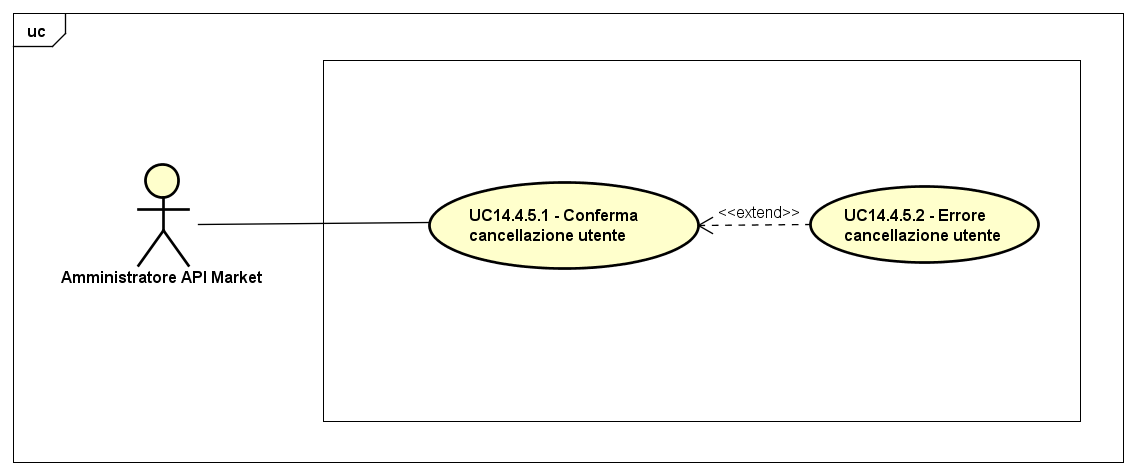
\includegraphics[scale=0.45]{UML/UC14_4_5.png}
	\caption{UC14.4.5: Cancellazione utente}
\end{figure}

\begin{minipage}{\linewidth}
	\begin{tabular}{ l | p{11cm}}
		\hline
		\rowcolor{Gray}
		\multicolumn{2}{c}{UC14.4.5 - Cancellazione utente} \\
		\hline
		\textbf{Attori} & Amministratore API Market \\
		\textbf{Descrizione} & L'attore imposta lo status dell'utente scelto come cancellato \\
		\textbf{Pre-Condizioni} & L'attore si trova nella schermata relativa all'amministrazione dell'applicazione web ed ha scelto un utente da moderare \\
		\textbf{Post-Condizioni} & L'attore ha impostato lo status dell'utente scelto come cancellato \\
		\textbf{Scenario Principale} & 
		\begin{enumerate*}[label=(\arabic*.),itemjoin={\newline}]
			\item L'attore può confermare la cancellazione dell'utente scelto (UC14.4.5.1)
		\end{enumerate*}\\
		\textbf{Scenari Alternativi} & 
		\begin{enumerate*}[label=(\arabic*.),itemjoin={\newline}]
			\item L'attore, dopo aver confermato la cancellazione dell'utente scelto, può visualizzare un messaggio di errore informativo e la cancellazione non avviene (UC14.4.5.2)
		\end{enumerate*}\\
	\end{tabular}
\end{minipage}

\subparagraph{Caso d'uso UC14.4.5.1: Conferma cancellazione utente}
\label{UC14_4_5_1}

\begin{minipage}{\linewidth}
	\begin{tabular}{ l | p{11cm}}
		\hline
		\rowcolor{Gray}
		\multicolumn{2}{c}{UC14.4.5.1 - Conferma cancellazione utente} \\
		\hline
		\textbf{Attori} & Amministratore API Market \\
		\textbf{Descrizione} & L'attore conferma la cancellazione dell'utente scelto e visualizza un messaggio di successo \\
		\textbf{Pre-Condizioni} & L'attore si trova nella schermata relativa all'amministrazione dell'applicazione web ed ha scelto un utente da moderare \\
		\textbf{Post-Condizioni} & L'attore ha confermato la cancellazione dell'utente scelto \\
		\textbf{Scenario Principale} & 
		\begin{enumerate*}[label=(\arabic*.),itemjoin={\newline}]
			\item L'attore conferma la cancellazione dell'utente scelto e visualizza un messaggio di successo
		\end{enumerate*}\\
	\end{tabular}
\end{minipage}

\subparagraph{Caso d'uso UC14.4.5.2: Errore cancellazione utente}
\label{UC14_4_5_2}

\begin{minipage}{\linewidth}
	\begin{tabular}{ l | p{11cm}}
		\hline
		\rowcolor{Gray}
		\multicolumn{2}{c}{UC14.4.5.2 - Errore cancellazione utente} \\
		\hline
		\textbf{Attori} & Amministratore API Market \\
		\textbf{Descrizione} & L'attore visualizza un messaggio di errore informativo e la cancellazione dell'utente scelto non avviene \\
		\textbf{Pre-Condizioni} & L'attore ha confermato la cancellazione dell'utente scelto ma si è verificato un errore \\
		\textbf{Post-Condizioni} & L'attore ha visualizzato un messaggio di errore informativo \\
		\textbf{Scenario Principale} & 
		\begin{enumerate*}[label=(\arabic*.),itemjoin={\newline}]
			\item L'attore può visualizzare un messaggio di errore informativo e la cancellazione dell'utente scelto non avviene
		\end{enumerate*}\\
	\end{tabular}
\end{minipage}